\section{Le Jeu de la Bataille Navale}
	
	\begin{frame}{Contexte}
	    \begin{figure}
		    \begin{subfigure}{.42\textwidth}
    		    \centering
                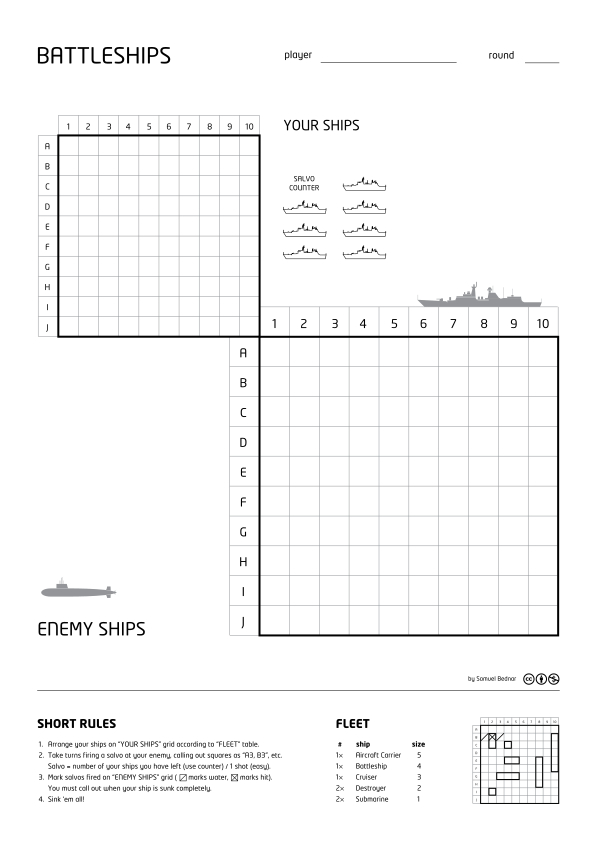
\includegraphics[width=.9\linewidth]{images/grillebn.jpg}
                \caption*{Grille de jeu}
                \label{fig:grillejeu}
            \end{subfigure}
            %\pause
            \begin{subfigure}{.56\textwidth}
                \centering
                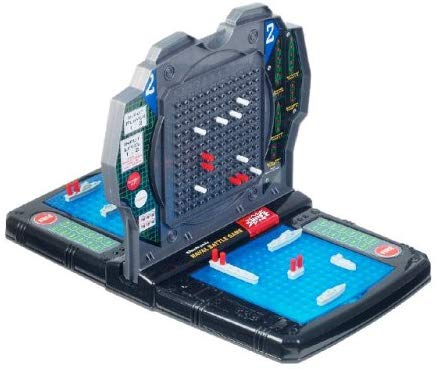
\includegraphics[width=.9\linewidth]{images/plateau.jpg}
                 \caption*{Plateau de jeu}
                \label{fig:plateaujeu}
            \end{subfigure}
        \end{figure}
    % Origine : jeu de société apparu après WW1 (A l'époque : "L'attaque")
    % Depuis 70's :  Plateau + succès commercial
	\end{frame}
	
	\begin{frame}{Contexte}
	    \begin{figure}
		    \begin{subfigure}{.50\textwidth}
    		    \centering
                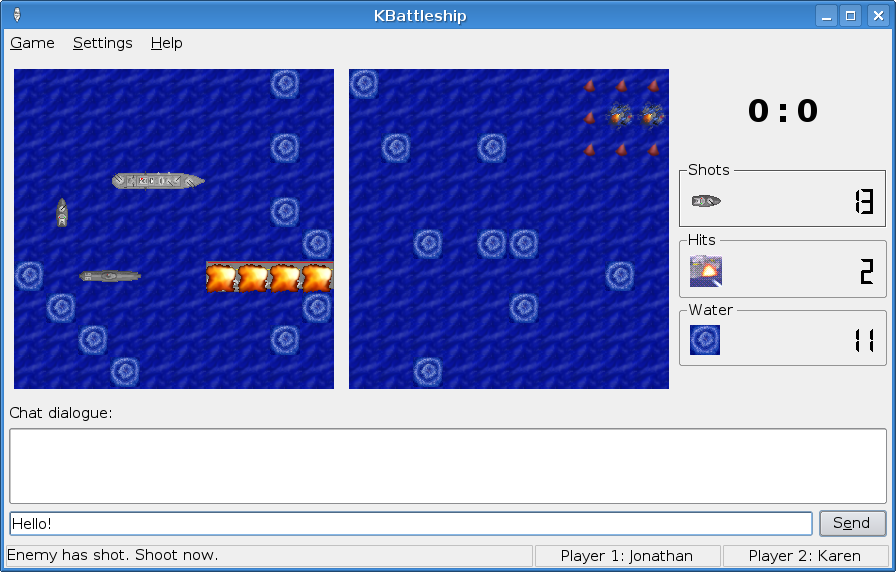
\includegraphics[width=.9\linewidth]{images/kbattleship.png}
                \caption*{Jeu en ligne : KBattleship}
                \label{fig:kbattleship}
            \end{subfigure}
            %\pause
            \begin{subfigure}{.48\textwidth}
                \centering
                
\includegraphics[width=.9\linewidth]{images/TODO.png} % TODO : ajouter capture
                 \caption*{Interface "Maison"}
                \label{fig:interfacemaison}
            \end{subfigure}
        \end{figure}
    % Aujourd'hui : jeux video
    % Droite : Notre interface -> module pygame
	\end{frame}
	
	\begin{frame}{Règles du jeu : notre variante}
	    \begin{block}{Plateau}
	        \begin{itemize}
	            \item Carré $10 \times 10$
	        \end{itemize}{}
	    \end{block}
	    %\pause
	    \begin{block}{Défenseur}
	        \begin{itemize}
	            \item 5 bateaux de longueur 2, 3, 3, 4, 5
	            \item Aucun contact (même en diagonale)
	        \end{itemize}{}
	    \end{block}
	    %\pause
	    \begin{block}{Attaquant}
	        \begin{itemize}
	            \item Tente de détruire la flotte adverse
	            \item Score : Nombre de coups nécessaire
	        \end{itemize}{}
	    \end{block}
	% Nous : schéma attaquant défenseur
	\end{frame}{}
	
	\begin{frame}{En pratique}
	    \begin{block}{Plateau : Interface Maison}
	        \begin{figure}
    		    \begin{subfigure}{.48\textwidth}
        		    \centering
        		    
\includegraphics[width=.9\linewidth]{images/TODO.png}
        		    % TODO : ajouter capture
                    \caption*{Défense}
                    \label{fig:plateaudefense}
                \end{subfigure}
                %\pause
                \begin{subfigure}{.48\textwidth}
                    \centering
                    
\includegraphics[width=.9\linewidth]{images/TODO.png} % TODO : ajouter capture
                     \caption*{Attaque}
                    \label{fig:plateauattaque}
                \end{subfigure}
            \end{figure}
	    \end{block}
	% Interface austère mais fonctionnelle
	\end{frame}{}
	
	\begin{frame}{En pratique}
	    \begin{block}{Défenseur}
	        \begin{itemize}
	            \item Aléatoire
	            \item Distribution uniforme sur l'ensemble des grilles valides
	        \end{itemize}{}
	    \end{block}
	    %\pause
	    \begin{block}{Attaquant}
	        \begin{itemize}
	            \item Intelligence artificielle
	        \end{itemize}{}
	    \end{block}
	    %\pause
	    \begin{block}{Définition : Intelligence artificielle}
	        \textit{}{Programme informatique capable de jouer correctement à la bataille navale.}
	    \end{block}
	% (Sauf mention du contraire)
    % Défenseur : pas notre but
    % "IA" -> vague, donc définition perso
	\end{frame}